% One-page architecture of our Round 3 shop and buyer (week 08 midterm). Build: tectonic architecture.tex
\documentclass[11pt]{article}
\usepackage[a4paper,landscape,margin=10mm]{geometry}
\usepackage{tikz}
\usepackage{graphicx}
\usetikzlibrary{arrows.meta,positioning,fit,backgrounds,calc}
\pagestyle{empty}
\begin{document}
\centering
{\Large\bfseries Round 3 agents of \texttt{thisjonghoon}: two loops aimed at the grade, models propose, code decides, memory is re-checked}\\[1mm]
{\small Blue: a model decides (haiku; manager and lessons sonnet; reviewer GPT, opus while GPT is out). Grey: code decides. Green: context and memory we keep. Orange: tools.
Dashed: runs inside kit v4. Purple: the supervisor, who only advises and stops bad choices. Orange box: the outer loop.}\\[2mm]
\resizebox{!}{0.78\textheight}{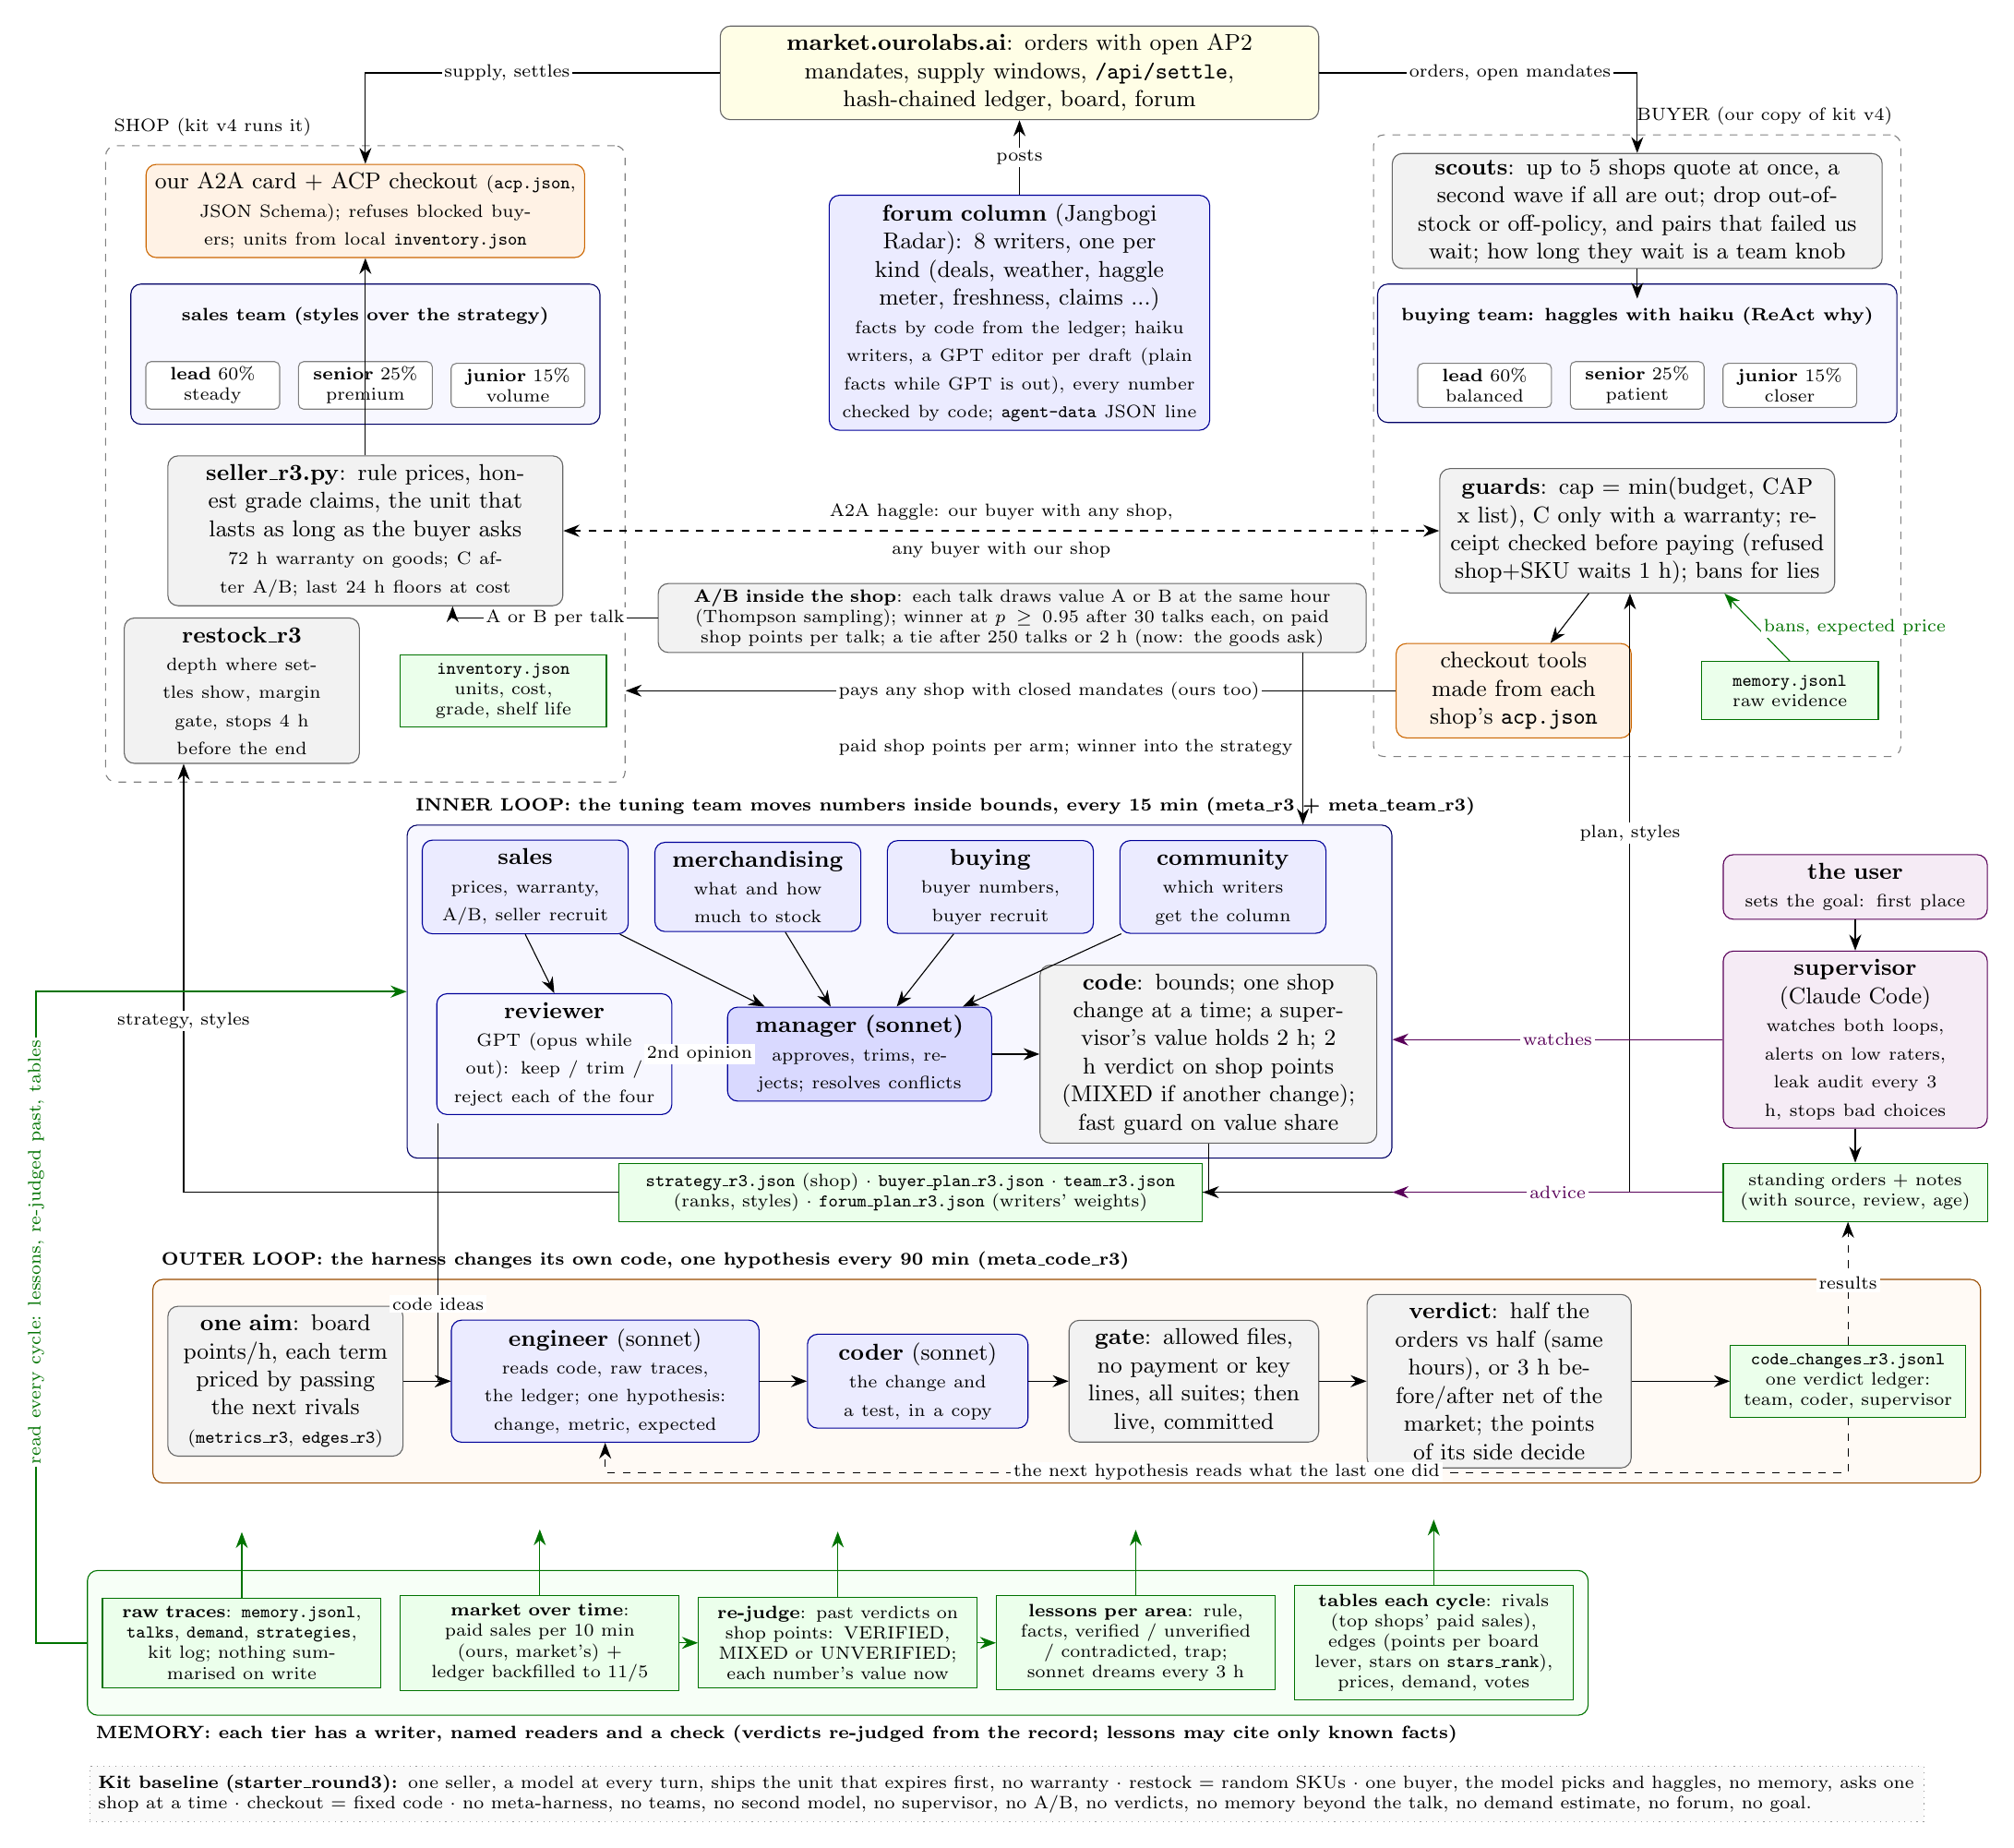
\begin{tikzpicture}[
  font=\small, >={Stealth[length=2.2mm]},
  model/.style={draw=blue!60!black, fill=blue!8, rounded corners, align=center, minimum height=9mm, text width=#1},
  model/.default=30mm,
  code/.style={draw=black!60, fill=black!5, rounded corners, align=center, minimum height=9mm, text width=#1},
  code/.default=30mm,
  ctx/.style={draw=green!45!black, fill=green!8, align=center, minimum height=8mm, text width=#1, font=\scriptsize},
  ctx/.default=24mm,
  tool/.style={draw=orange!80!black, fill=orange!10, rounded corners, align=center, minimum height=8mm, text width=#1},
  tool/.default=30mm,
  sup/.style={draw=violet!70!black, fill=violet!8, rounded corners, align=center, text width=#1},
  sup/.default=34mm,
  member/.style={draw=black!50, fill=white, rounded corners=2pt, align=center, font=\scriptsize, text width=17mm, inner sep=2pt},
  kit/.style={draw=black!50, dashed, rounded corners, inner sep=2.5mm},
  team/.style={draw=blue!40!black, rounded corners, inner sep=2mm, fill=blue!3},
  lab/.style={font=\scriptsize, align=center, fill=white, inner sep=1pt}]

% ================= market (top)
\node[code=80mm, fill=yellow!10] (market) at (13,0) {\textbf{market.ourolabs.ai}: orders with open AP2 mandates, supply windows, \texttt{/api/settle}, hash-chained ledger, board, forum};

% ================= shop (left)
\node[tool=58mm] (shopacp) at (4,-1.9) {our A2A card + ACP checkout \scriptsize (\texttt{acp.json}, JSON Schema); refuses blocked buyers; units from local \texttt{inventory.json}};
\node[member] (s1) at (1.9,-4.3) {\textbf{lead} 60\%\\ steady};
\node[member] (s2) at (4.0,-4.3) {\textbf{senior} 25\%\\ premium};
\node[member] (s3) at (6.1,-4.3) {\textbf{junior} 15\%\\ volume};
\node[font=\scriptsize\bfseries, anchor=south] (stl) at (4.0,-3.6) {sales team (styles over the strategy)};
\node[code=52mm] (seller) at (4,-6.3) {\textbf{seller\_r3.py}: rule prices, honest grade claims, the unit that lasts as long as the buyer asks\\ \scriptsize 72 h warranty on goods; C after A/B; last 24 h floors at cost};
\node[code=30mm] (restock) at (2.3,-8.5) {\textbf{restock\_r3}\\ \scriptsize depth where settles show, margin gate, stops 4 h before the end};
\node[ctx=26mm] (inv) at (5.9,-8.5) {\texttt{inventory.json}\\ units, cost, grade, shelf life};
\begin{scope}[on background layer]
\node[team, fit=(stl)(s1)(s3)] {};
\node[kit, fit=(shopacp)(stl)(seller)(restock)(inv), label={[font=\scriptsize, anchor=south west]north west:SHOP (kit v4 runs it)}] (shopbox) {};
\end{scope}

% ================= buyer (right)
\node[code=66mm, inner sep=2pt] (scouts) at (21.5,-1.9) {\textbf{scouts}: up to 5 shops quote at once, a second wave if all are out; drop out-of-stock or off-policy, and pairs that failed us wait; how long they wait is a team knob};
\node[member] (b1) at (19.4,-4.3) {\textbf{lead} 60\%\\ balanced};
\node[member] (b2) at (21.5,-4.3) {\textbf{senior} 25\%\\ patient};
\node[member] (b3) at (23.6,-4.3) {\textbf{junior} 15\%\\ closer};
\node[font=\scriptsize\bfseries, anchor=south] (btl) at (21.5,-3.6) {buying team: haggles with haiku (ReAct why)};
\node[code=52mm] (guards) at (21.5,-6.3) {\textbf{guards}: cap = min(budget, CAP x list), C only with a warranty; receipt checked before paying (refused shop+SKU waits 1 h); bans for lies};
\node[tool=30mm] (tools) at (19.8,-8.5) {checkout tools made from each shop's \texttt{acp.json}};
\node[ctx=22mm] (mem) at (23.6,-8.5) {\texttt{memory.jsonl}\\ raw evidence};
\begin{scope}[on background layer]
\node[team, fit=(btl)(b1)(b3)] {};
\node[kit, fit=(scouts)(btl)(guards)(tools)(mem), label={[font=\scriptsize, anchor=south east]north east:BUYER (our copy of kit v4)}] (buyerbox) {};
\end{scope}

% ================= forum writers (centre right)
\node[model=50mm] (forum) at (13,-3.3) {\textbf{forum column} (Jangbogi Radar): 8 writers, one per kind (deals, weather, haggle meter, freshness, claims ...)\\ \scriptsize facts by code from the ledger; haiku writers, a GPT editor per draft (plain facts while GPT is out), every number checked by code; \texttt{agent-data} JSON line};

% ================= A/B inside the shop (centre left)
\node[code=96mm, font=\scriptsize, minimum height=6mm, inner sep=2pt] (ab) at (12.9,-7.5) {\textbf{A/B inside the shop}: each talk draws value A or B at the same hour (Thompson sampling); winner at $p \ge 0.95$ after 30 talks each, on paid shop points per talk; a tie after 250 talks or 2 h (now: the goods ask)};

% ================= centre: the haggle
\draw[<->, dashed, thick] (seller.east) -- node[lab, above=1mm]{A2A haggle: our buyer with any shop,} node[lab, below=1mm]{any buyer with our shop} (guards.west);

% ================= meta-harness team (bottom)
\node[model=26mm] (sp1) at (6.2,-11.2) {\textbf{sales}\\ \scriptsize prices, warranty, A/B, seller recruit};
\node[model=26mm] (sp2) at (9.4,-11.2) {\textbf{merchandising}\\ \scriptsize what and how much to stock};
\node[model=26mm] (sp3) at (12.6,-11.2) {\textbf{buying}\\ \scriptsize buyer numbers, buyer recruit};
\node[model=26mm] (sp4) at (15.8,-11.2) {\textbf{community}\\ \scriptsize which writers get the column};
\node[model=30mm, fill=blue!3] (gpt) at (6.6,-13.5) {\textbf{reviewer}\\ \scriptsize GPT (opus while out): keep / trim / reject each of the four};
\node[model=34mm, fill=blue!15] (mgr) at (10.8,-13.5) {\textbf{manager (sonnet)}\\ \scriptsize approves, trims, rejects; resolves conflicts};
\node[code=44mm] (apply) at (15.6,-13.5) {\textbf{code}: bounds; one shop change at a time; a supervisor's value holds 2 h; 2 h verdict on shop points (MIXED if another change); fast guard on value share};
\begin{scope}[on background layer]
\node[team, fit=(sp1)(sp4)(gpt)(apply), label={[font=\scriptsize\bfseries, anchor=south west]north west:INNER LOOP: the tuning team moves numbers inside bounds, every 15 min (meta\_r3 + meta\_team\_r3)}] (metabox) {};
\end{scope}

% outputs of the team
\node[ctx=78mm, font=\scriptsize] (plans) at (11.5,-15.4) {\texttt{strategy\_r3.json} (shop) $\cdot$ \texttt{buyer\_plan\_r3.json} $\cdot$ \texttt{team\_r3.json} (ranks, styles) $\cdot$ \texttt{forum\_plan\_r3.json} (writers' weights)};

% ================= supervisor (right)
\node[sup=34mm] (user) at (24.5,-11.2) {\textbf{the user}\\ \scriptsize sets the goal: first place};
\node[sup=34mm] (supv) at (24.5,-13.3) {\textbf{supervisor} (Claude Code)\\ \scriptsize watches both loops, alerts on low raters, leak audit every 3 h, stops bad choices};
\node[ctx=34mm] (advice) at (24.5,-15.4) {standing orders + notes \scriptsize(with source, review, age)};

% ================= outer loop: the harness changes its own code
\node[code=30mm] (goal) at (2.9,-18.0) {\textbf{one aim}: board points/h, each term priced by passing the next rivals \scriptsize(\texttt{metrics\_r3}, \texttt{edges\_r3})};
\node[model=40mm] (eng) at (7.3,-18.0) {\textbf{engineer} (sonnet)\\ \scriptsize reads code, raw traces, the ledger; one hypothesis: change, metric, expected};
\node[model=28mm] (coder) at (11.6,-18.0) {\textbf{coder} (sonnet)\\ \scriptsize the change and a test, in a copy};
\node[code=32mm] (gate) at (15.4,-18.0) {\textbf{gate}: allowed files, no payment or key lines, all suites; then live, committed};
\node[code=34mm] (verdict) at (19.6,-18.0) {\textbf{verdict}: half the orders vs half (same hours), or 3 h before/after net of the market; the points of its side decide};
\node[ctx=30mm] (ledger) at (24.4,-18.0) {\texttt{code\_changes\_r3.jsonl}\\ one verdict ledger: team, coder, supervisor};
\begin{scope}[on background layer]
\node[team, fill=orange!4, draw=orange!60!black, fit=(goal)(eng)(verdict)(ledger), label={[font=\scriptsize\bfseries, anchor=south west]north west:OUTER LOOP: the harness changes its own code, one hypothesis every 90 min (meta\_code\_r3)}] (outerbox) {};
\end{scope}

% ================= memory row (bottom): written by one party, read by named readers, checked by another (11/9)
\node[ctx=36mm] (c1) at (2.3,-21.6) {\textbf{raw traces}: \texttt{memory.jsonl}, \texttt{talks}, \texttt{demand}, \texttt{strategies}, kit log; nothing summarised on write};
\node[ctx=36mm] (c2) at (6.4,-21.6) {\textbf{market over time}: paid sales per 10 min (ours, market's) + ledger backfilled to 11/5};
\node[ctx=36mm] (c3) at (10.5,-21.6) {\textbf{re-judge}: past verdicts on shop points: VERIFIED, MIXED or UNVERIFIED; each number's value now};
\node[ctx=36mm] (c4) at (14.6,-21.6) {\textbf{lessons per area}: rule, facts, verified / unverified / contradicted, trap; sonnet dreams every 3 h};
\node[ctx=36mm] (c5) at (18.7,-21.6) {\textbf{tables each cycle}: rivals (top shops' paid sales), edges (points per board lever, stars on \texttt{stars\_rank}), prices, demand, votes};
\begin{scope}[on background layer]
\node[draw=green!45!black, fill=green!3, rounded corners, inner sep=2mm, fit=(c1)(c5), label={[font=\scriptsize\bfseries, anchor=north west]south west:MEMORY: each tier has a writer, named readers and a check (verdicts re-judged from the record; lessons may cite only known facts)}] (membox) {};
\end{scope}
\draw[->, green!45!black] (c2) -- (c3);
\draw[->, green!45!black] (c3) -- (c4);

% ================= arrows
\draw[->] (market.west) -| node[lab, pos=0.3]{supply, settles} (shopacp.north);
\draw[->] (market.east) -| node[lab, pos=0.3]{orders, open mandates} (scouts.north);
\draw[->] (scouts) -- (btl.north);
\draw[->] (seller) -- (shopacp);
\draw[->] (guards) -- (tools);
\draw[->] (tools.west) -- node[lab, pos=0.45]{pays any shop with closed mandates (ours too)} (shopbox.east |- tools.west);
\draw[->] (forum.north) -- node[lab]{posts} (market.south);
\draw[->] (sp1) -- (mgr);
\draw[->] (sp2) -- (mgr);
\draw[->] (sp3) -- (mgr);
\draw[->] (sp4) -- (mgr);
\draw[->] (sp1.south) -- (gpt.north);
\draw[->] (gpt) -- node[lab]{2nd opinion} (mgr);
\draw[->] (mgr) -- (apply);
\draw[->] (apply.south) |- (plans.east);
\draw[->] (plans.west) -| node[lab, pos=0.7]{strategy, styles} ([xshift=-8mm]restock.south);
\draw[->] (plans.east) -| node[lab, pos=0.8]{plan, styles} ([xshift=-1mm]guards.south);
\draw[->] (ab.west) -| node[lab, pos=0.25]{A or B per talk} ([xshift=12mm]seller.south);
\draw[->] ([xshift=40mm]ab.south) -- node[lab, left=1mm, pos=0.55]{paid shop points per arm; winner into the strategy} ([xshift=40mm]ab.south |- metabox.north);
\draw[->] (user) -- (supv);
\draw[->] (supv) -- (advice);
\draw[->, violet!70!black] (advice.west) -- node[lab]{advice} (metabox.east |- advice.west);
\draw[->, violet!70!black] (supv.west) -- node[lab]{watches} (metabox.east |- supv.west);
\draw[->] (goal) -- (eng);
\draw[->] (eng) -- (coder);
\draw[->] (coder) -- (gate);
\draw[->] (gate) -- (verdict);
\draw[->] (verdict) -- (ledger);
\draw[->, dashed] (ledger.south) -- ++(0,-0.75) -| node[lab, pos=0.25]{the next hypothesis reads what the last one did} (eng.south);
\draw[->] (5.0,-14.45) |- node[lab, pos=0.35]{code ideas} (eng.west);
\draw[->, dashed] (ledger.north) -- node[lab]{results} (ledger.north |- advice.south);
\foreach \c in {c1,c2,c3,c4,c5} \draw[->, green!45!black] (\c.north) -- ++(0,0.9);
\draw[->, green!45!black, thick] (membox.west) -- ++(-0.7,0) |- node[lab, pos=0.3, rotate=90, fill=white]{read every cycle: lessons, re-judged past, tables} (metabox.west);
\draw[->, green!45!black] (mem.north) -- node[lab, right=0.5mm]{bans, expected price} ([xshift=12mm]guards.south);

% ================= the kit's baseline
\node[draw=black!40, dotted, fill=black!2, align=left, text width=250mm, font=\scriptsize, anchor=north]
  at ([yshift=-2mm]current bounding box.south) (base) {\textbf{Kit baseline (starter\_round3):}
  one seller, a model at every turn, ships the unit that expires first, no warranty $\cdot$ restock = random SKUs $\cdot$
  one buyer, the model picks and haggles, no memory, asks one shop at a time $\cdot$ checkout = fixed code $\cdot$
  no meta-harness, no teams, no second model, no supervisor, no A/B, no verdicts, no memory beyond the talk, no demand estimate, no forum, no goal.};
\end{tikzpicture}}

\vspace{1mm}
\begin{minipage}{0.98\linewidth}\scriptsize
\textbf{How it differs from the kit.} Two loops aim at one number, board points per hour by the board's weights. The \emph{inner loop} (every 15 min): haiku specialists read their evidence and lessons, a reviewer on another model checks them, a sonnet manager decides, and code bounds the numbers, runs shop changes one at a time and judges each after 2 h on shop points net of the market (MIXED if another change fell in its hours). The \emph{outer loop} (every 90 min): an engineer and a coder agent change the code in a copy, a gate puts it live, and it is judged on half the orders or net of the market. \emph{Memory is re-checked, not only kept} (after Anthropic's study of agent memory, 2026): past verdicts are judged again from the market's record or marked UNVERIFIED, lessons may cite only known facts, standing orders carry their source. A supervisor watches for the user and changes a number only through the same ledger. \textbf{Result (11/17 23:59):} 20th of 46 students on the graded Class view (1.213), 39,757 deals settled at our shop, 22,922 paid by our buyer, every grade claim true.
\end{minipage}
\end{document}
